%%
%% THESIS/DISSERTATION TEMPLATE FOR THE UNIVERSITY OF ALABAMA.
%%
%% This example is written by Paul Kilgo. It highlights all the (few) features
%% of uathesis.cls
%%

%% Use one of the following if writing a thesis/dissertation.
% \documentclass[thesis]{uathesis}
\documentclass[dissertation]{uathesis}

%% Basic packages you'll probably want to use.
\usepackage{graphicx}                 %% For using \includegraphics{}
\usepackage{cite}                     %% For sorting/collapsing citations.
\usepackage{color}                    %% For colors used in listings.
\usepackage{listings}                 %% Code listings (for engineers)
\usepackage[numbers]{natbib}
%% Includes
\newacronym{tmi}{TMI}{Too Much Information}
\newacronym{lol}{LOL}{Laughing Out Loud}
\newacronym{rotflol}{ROTFLOL}{Rolling On The Floor Laughing Out Loud}

\newglossaryentry{beta}
{
  name={\ensuremath{\beta}},
  description={The Greek Letter Beta},
  sort=beta
}

\newglossaryentry{alpha}
{
  name={\ensuremath{\alpha}},
  description={The Greek Letter Alpha},
  sort=alpha
}

% TODO: If you have any special commands defined, include them here.
\usepackage[titletoc]{appendix}%

%% Required parameters (these default to undefined)
\author{Joe Somebody}       %% Your name!
\adviser{The Boss}   %% Your adviser/committee chair!

%% The people on your committee.
%% Use \and to break them up between lines.
\committee{
  Andy Smith \and
  Billy Smith \and
  Carl Smith
}

%% Note the use of \and to create line breaks and the
%% inverted pyramid style requested by the graduate school.
%% You have to do this manually. Sorry.
\title{Title of the thesis: the top line should be the longest \and
  the middle one is second longest \and
  and the last is shortest}

\degree{Doctor of Philosophy}   %% Change to suit your degree.
\department{Computer Science}   %% Change to suit your department.

%% These are body text paragraphs to be placed in the front matter.
\abstract{
  There is such a thing as \gls{tmi}. My brother once said that \gls{tmi}
  is what drives the world, some times causing fits of \gls{lol}. If one
  is to get in a especially deep fit of the \glspl{lol}, then one could
  find oneself \gls{rotflol}.

  By the way, \gls{alpha} and \gls{beta} are Greek letters.
}

\dedication{
  Type or input{} your dedication here.
}

\acknowledgments{
  Type or input{} your acknowledgments here.
}

%% Optional parameters. The default usage is shown.
\university{The University of Alabama}
\school{Graduate School}
\gradyear{\the\year}
\place{Tuscaloosa, Alabama}

\begin{document}

%% Makes the title, abstract, dedication, table of contents, etc.
%% Must be before \begin{body}
\makefrontmatter

%% BODY PORTION
%% The bulk of your thesis.
%% Begin your \chapter's here.

\begin{body}

%% Body chapters.
\chapter{INTRODUCTION}

Take a look at Figure \ref{fig:shapes}. It has some shapes. They're very
complex and interesting shapes. I could gaze at them for hours.

\begin{figure}
  \centering
  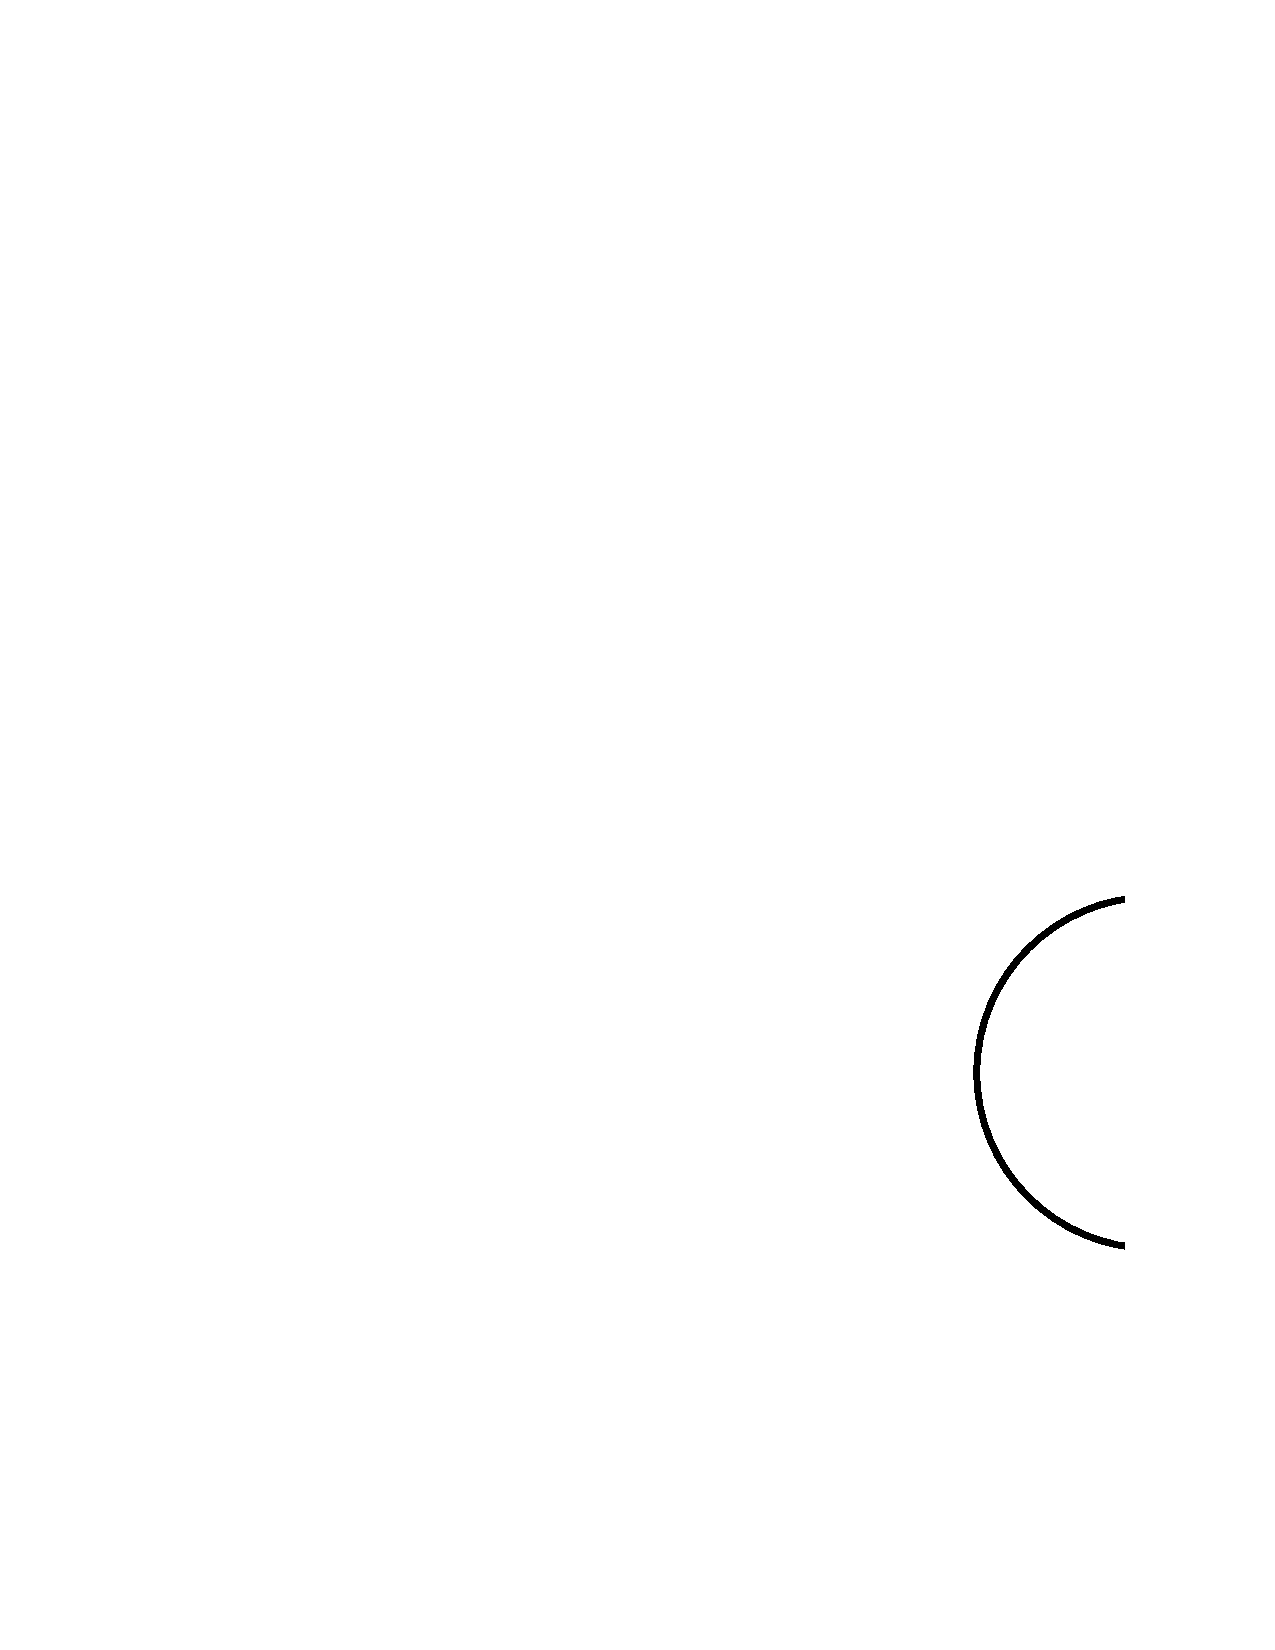
\includegraphics[width=5.0in]{fig/shapes.pdf}
  \caption{Some shapes which I find very interesting. (has longer line than 1, so that we can try it in LoF.}
  \label{fig:shapes}
\end{figure}

\chapter{LITERATURE REVIEW}
Type or input{} a chapter. \cite{rocket-themoon2167}

\chapter{APPROACH (BECAUSE A LONGER-THAN-1-LINE CHAPTER TITLE IS IMPORTANT)}
Take a look at Table \ref{tab:love-shapes}. It shows how much I love certain
shapes.

\begin{table}
  \centering
  \begin{tabular}{|c|c|}
  Name & Units of Love \\ \hline
  Circle   &  27 \\
  Square   &  42 \\
  Triangle &  12 \\
\end{tabular}

  \caption{Shapes and corresponding love in Love Standard Units (LSU).}
  \label{tab:love-shapes}
\end{table}

\chapter{EXPERIMENT}
Type or input{} a chapter. \cite{rocket-themoon2167}

\chapter{DISCUSSION}
Type or input{} a chapter. \cite{rocket-themoon2167}

\chapter{CONCLUSION}
Type or input{} a chapter. \cite{rocket-themoon2167}

%% Currently adding the references to the table of contents is not automatic
%% So we are forced to do it manually.

%% TODO: This is not a fix. This line has to come after the \chapter command
%% in order for the correct page to be inferred for the table of contents.
\renewcommand{\bibsection}{\topskip=1in\chapter*{REFERENCES}\topskip=0in \addcontentsline{toc}{chapter}{REFERENCES}}

%% Generates the bibliography.
\bibliographystyle{uathesis-plain}
\bibliography{thesis-template}

\begin{appendices}
\addtocontents{toc}{\setlength{\cftchapnumwidth}{1em}}
\renewcommand{\appendixname}{APPENDIX}
\addtocontents{toc}{\setcounter{tocdepth}{0}}
\addtocontents{toc}{\protect\renewcommand{\protect\cftchappresnum}{}}

\chapter{A BIG APPENDIX}

\end{appendices}

\end{body}
\end{document}
